\section{Comparisons with Previous Studies}

\begin{figure}[t]
\centering
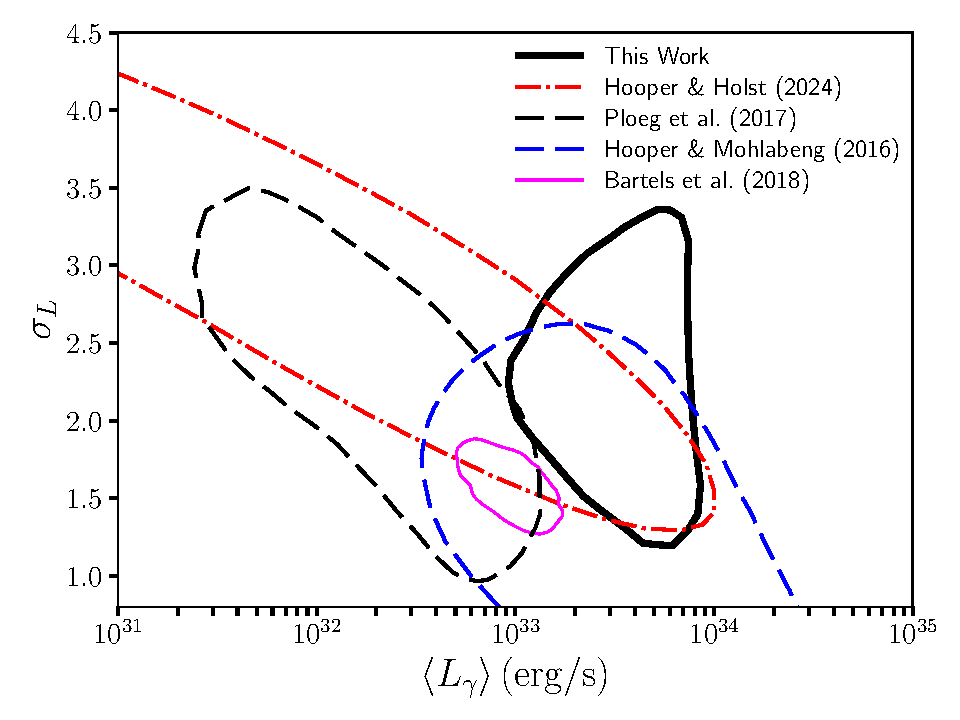
\includegraphics[width=0.66\textwidth]{img/contours_compare.pdf}
\caption{A comparison of the $2\sigma$ constraints on the MSP gamma-ray luminosity found in this study (for the best-fitting case of $\langle N_{\rm MSP}\rangle = R_{\rm MSP} \, \Gamma_e^{0.7} +R'_{\rm MSP} \, L_V$) to those published in previous studies of MSPs in the Galactic Plane. The luminosity function preferred by our analysis is in good agreement with those derived by Holst and Hooper~\cite{Holst:2024fvb}, and by Hooper and Mohlabeng~\cite{Hooper:2016rap}, but favor somewhat larger values for the average MSP luminosity than Ploeg {\it et al.}~\cite{Ploeg:2017vai}, or Bartels {\it et al.}~\cite{Bartels:2018xom}.}
\label{fig:compare}
\end{figure}

A number of previous studies have attempted to measure or constrain the gamma-ray luminosity function of MSPs~\cite{Holst:2024fvb,Cholis:2014noa,Hooper:2016rap,Hooper:2015jlu,Bartels:2018xom,Ploeg:2017vai,Ploeg:2020jeh}). In Fig.~\ref{fig:compare}, we compare the results of this study (for the best-fitting case of $\langle N_{\rm MSP}\rangle = R_{\rm MSP} \, \Gamma_e^{0.7} +R'_{\rm MSP} \, L_V$) with those published in previous studies of the MSP population within the Galactic Plane. The luminosity function preferred by our analysis is in good agreement with those recently derived by Holst and Hooper~\cite{Holst:2024fvb},  and previously by Hooper and Mohlabeng~\cite{Hooper:2016rap}. Our results, however, favor somewhat larger values of the average MSP luminosity, $\langle L_{\gamma}\rangle$, than the analyses of Ploeg {\it et al.}~\cite{Ploeg:2017vai} or Bartels {\it et al.}~\cite{Bartels:2018xom}.

 

We note that the analysis of Bartels {\it et al.}~\cite{Bartels:2018xom} made use of pulsar distance measurements, which are
often subject to significant and difficult to quantify systematic uncertainties. For most pulsars, distance estimates are derived
from measurements of their dispersion measure (ie., the frequency-dependent time delay of the radio pulses, which can be used to determine the column density of free electrons along the pulsar’s line-of-sight). When the dispersion measure of a pulsar is combined with a model of the free electron distribution, one can obtain an estimate of its distance. Such estimates are known to vary significantly, however, depending on the electron distribution model that is adopted~\cite{Yao:2017kcp,Cordes:2002wz}, and sometimes disagree with more reliable parallax determinations by factors of up to $\sim 3$~\cite{Fermi-LAT:2023zzt}.

It is possible that the MSPs population found within globular clusters could feature a gamma-ray luminosity function that is different from those pulsars in the Galactic Plane. This could be motivated by the fact that globular clusters are known to contain an old stellar population, and their pulsars could plausibly have already lost much of rotational kinetic energy, compared to that of more recently formed MSPs. This difference, however, would lead us to expect MSPs in globular clusters to be systematically {\it fainter} than those in the Galactic Plane, which is opposite to that found in the studies of Ploeg {\it et al.}~\cite{Ploeg:2017vai} and Bartels {\it et al.}~\cite{Bartels:2018xom}.   

We can more directly compare our results to those of the 2016 analysis by Hooper and Linden~\cite{Hooper:2016rap}, which also studied MSPs in globular clusters, using in their case 7 years of Fermi data (compared to the 15.8 years of data used in this analysis). The 2016 study favored a MSP gamma-ray luminosity function with $\langle L_{\gamma} \rangle \sim (0.7-5) \times 10^{34} \, {\rm erg/s}$ and $\sigma_L \sim 1-3$. While the results presented here are statistically consistent with those of that study (at the approximately $\sim 2\sigma$ level), our analysis tends to prefer somewhat smaller values of $\langle L_{\gamma} \rangle$ and larger values of $R_{\rm MSP}$, by a factor of $\sim 2-8$. For a more detailed comparison, see Appendix \ref{sec:app-comparison}.

